\subsection{Map}\label{ssec:map}
The Map data type represents 2D spatial data such as images of the Sun and 
inner heliosphere. It provides a wrapper around a data array and its associated
spatial coordinates and other metadata. The \texttt{Map} class provides 
methods for typical operations on 2D data, 
such as rotation and re-sampling, and visualisation functionality.
The \texttt{Map} class
also provides a convenient interface for loading data from a variety of sources, typically
a FITS file as shown in Listing~\ref{code:aia_1}.

The architecture of the \texttt{Map} class consists of a template map called
\texttt{GenericMap}, which is a subclass of \texttt{astropy.nddata.NDData}. \texttt{NDData} is a 
generic wrapper around an \texttt{ndarray} with a \texttt{.meta} attribute to store metadata.
As \texttt{NDData} is currently still in development, \texttt{GenericMap} does not yet make full
use of its capabilities, but this inheritance structure provides 
for future integration of \texttt{Astropy}. In order to provide instrument- or
detector-specific integration, \texttt{GenericMap} is subclassed on creation. 
Each subclass of \texttt{GenericMap} can register with the \texttt{Map} creation function (\textit{i.e.}, factory)
by implementing a method that returns \texttt{True} if the metadata
in the file header matches
that instrument or detector.  This \texttt{Map} factory 
will then automatically return an instance of the specific \texttt{GenericMap} 
subclass. SunPy 0.4 has \texttt{Map} specialisations for the 
following instruments: 
\textit{YOHKOH/SXT}, \textit{SOHO/EIT} and \textit{LASCO}, \textit{RHESSI}, 
\textit{STEREO/EUVI} and \textit{COR}, \textit{HINODE/XRT},
\textit{PROBA2/SWAP}, \textit{SDO/AIA} and \textit{HMI}, 
and \textit{IRIS} SJI frames. 

The \texttt{Map} class stores standard metadata retrieved from the header of 
the image file in the \texttt{.meta} attribute and provides convenience 
properties for commonly accessed metadata: \textit{e.g.}, \texttt{.instrument}, 
\texttt{.wavelength} or \texttt{.coordinate\_system}. 
Listing \ref{code:aia_1} demonstrates the quick-plot functionality of 
\texttt{Map}; see Section \ref{subsec:Viz} for more discussion of plotting.

\begin{listing}[H]
\begin{minted}[bgcolor=bg]{pycon}
>>> import sunpy.map
>>> aiamap = sunpy.map.Map('aia_file.fits')
>>> aiamap.peek()
\end{minted}
\begin{center}
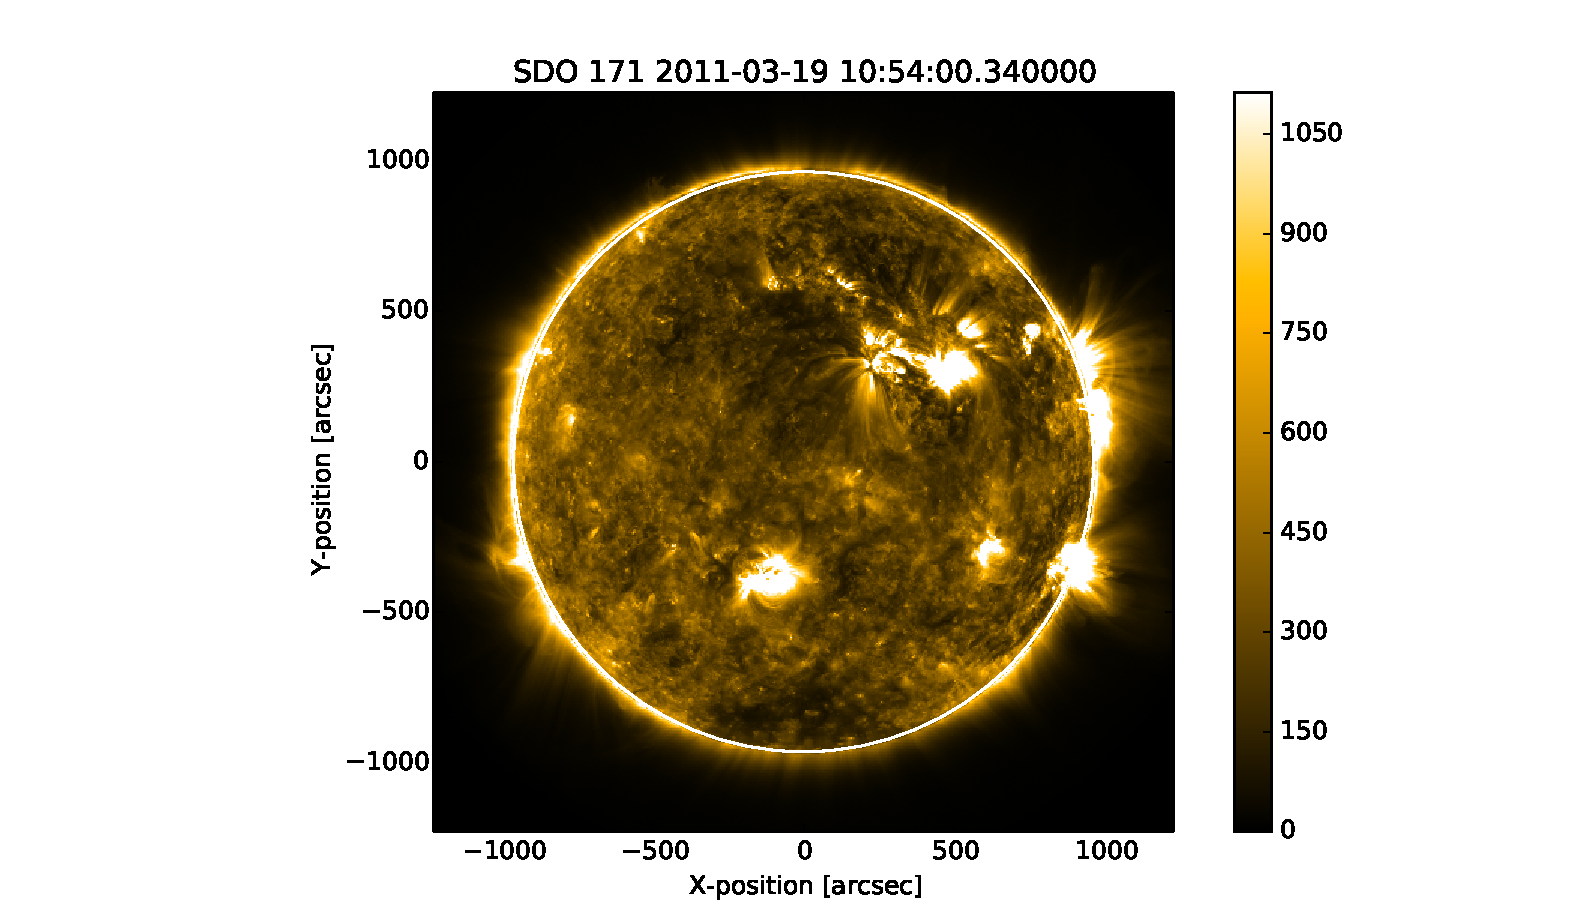
\includegraphics[width=0.8\columnwidth]{aia_map_example}
\end{center}
\caption{Example of the \texttt{AIAMap} specialisation of 
\texttt{GenericMap}. The Map is created from an \textit{AIA} FITS file,
and a quick-view plot is created.}
\label{code:aia_1}
\end{listing}

In addition to the data-type classes, the \texttt{map} sub-package provides two 
collection classes, \texttt{CompositeMap} and \texttt{MapCube}, for 
temporally and spatially aligned data respectively.
\texttt{CompositeMap} provides methods for overlaying spatially aligned 
data, with support for visualisation of images and contour lines overlaid 
upon each other.
\texttt{MapCube} 
provides methods for animation of its series of \texttt{Map} objects. 
Listings~\ref{code:compmap_1} and \ref{code:mapcube_1} show how to interact 
with these classes.
In addition, Listing~\ref{code:mapcube_2} shows how the \texttt{MapCube} 
classes interacts with the \texttt{animation} module to save a video.

\begin{listing}[H]
\begin{minted}[bgcolor=bg]{pycon}
>>> import matplotlib.pyplot as plt
>>> import sunpy.map
>>> compmap = sunpy.map.Map('aia_1600_image.fits', 'RHESSI_image.fits', 
...                         composite=True)
>>> compmap.set_levels(1, range(0,50,5), percent=True)
>>> compmap.set_colors(1, 'Reds_r')
#Plot the result and crop
>>> ax = plt.subplot()
>>> compmap.plot()
>>> ax.axis([200, 600, -600, -200])
>>> plt.show()
\end{minted}
\begin{center}
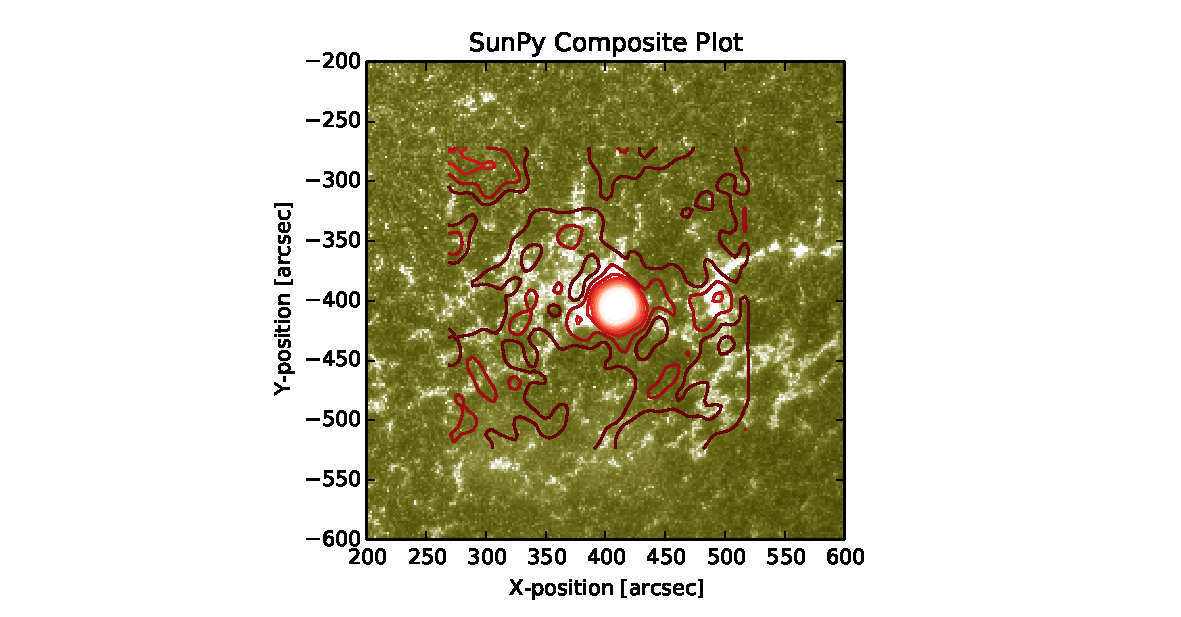
\includegraphics[width=0.8\columnwidth]{comp_map_example}
\end{center}
\caption{Example showing a \texttt{CompositeMap} plot and the integration with the \texttt{matplotlib.pyplot} interface.}
\label{code:compmap_1}
\end{listing}

%schriste - stuart, i agree if you want to remove the following two listings.
\begin{listing}[H]
\begin{minted}[bgcolor=bg]{pycon}
>>> import sunpy.map
>>> compmap = sunpy.map.Map('aia_lev1_171a_2014_01*fits', cube=True)
>>> compmap.peek()
\end{minted}
\begin{center}
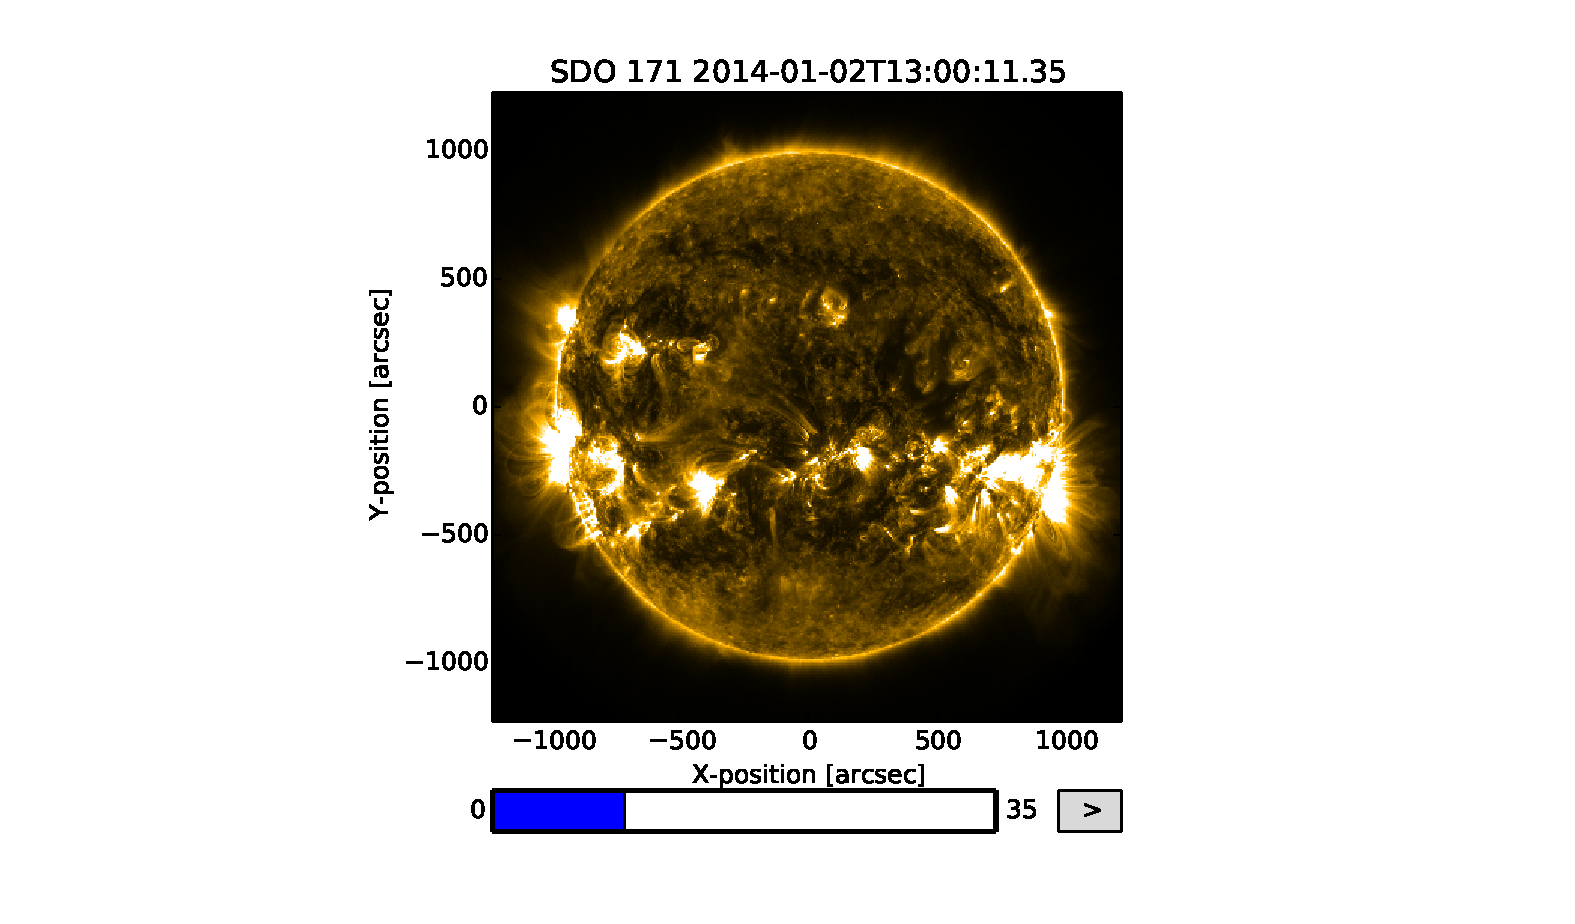
\includegraphics[width=0.8\columnwidth]{aia_cube_controls}
\end{center}
\caption{Example showing creation of a \texttt{MapCube} from a glob file search. The 
resultant plot makes use of \texttt{matplotlib}'s interactive widgets to allow scrolling 
through the \texttt{MapCube}.}
\label{code:mapcube_1}
\end{listing}

\begin{listing}[H]
\begin{minted}[bgcolor=bg]{pycon}
>>> import sunpy.map
>>> from matplotlib import animation
>>> mapc = sunpy.map.Map('aia_lev1_171a_2014_01*fits', cube=True)
>>> anim = mapc.plot()
>>> Writer = animation.writers['ffmpeg']
>>> writer = Writer(fps=10, metadata=dict(artist='SunPy'), bitrate=1800)
>>> anim.save('aia_cube.ogv')
\end{minted}
% In the above example, is Writer, writer clear? 
% Could we add more metadata to the movie? obs_date, instrument, etc...?
\caption{Example showing how to save a video animation from a \texttt{MapCube}, using 
\texttt{matplotlib}'s animation framework.}
\label{code:mapcube_2}
\end{listing}
